\section{Praktikos veiklos aprašymas}

\begin{activities}
    \veikla{Duomenų saugyklos pasirinkimas}
    \aprasymas{
        Peržiūrėtos organizacijoje naudojamos duomenų saugyklos. Atrinkti 3 galimi variantai:
        \begin{enumerate}
            \item \textit{S3 on-prem} -- duomenų saugykla, palaikanti S3 protokolą \angl{S3 Compatible Storage}. Ši saugykla veikia organizacijos valdomuose serveriuose, juos prižiūri IT infrastruktūros skyrius.
            % Issue URL: https://github.com/onlyidev/bachelor.practice/issues/5
            \item \textit{S3 Minio}~\cite{MinIOS3Compatible} -- duomenų saugykla, palaikanti S3 protokolą. Ši saugykla veikia konteinerizuotoje aplinkoje. Kiekviena sistema gali turėti savo \textit{Minio} komponentą ir ten kaupti duomenis. Tokiu atveju už šį komponentą atsakinga sistemą prižiūrinti komanda.
            % Issue URL: https://github.com/onlyidev/bachelor.practice/issues/4
            \item \textit{Failų serveris \angl{File Server}} -- duomenų saugykla, palaikanti SFTP \textit{(Secure File Transfer Protocol)}~\cite{krishnaSecureFileMulti2011}. Ši saugykla veikia organizacijos valdomuose serveriuose, juos prižiūri IT infrastruktūros skyrius.
        \end{enumerate}

        Dėl organizacijoje priimtos strategijos, failų serverio varianto buvo
        atsisakyta iškart. \textit{S3 Minio} variantas atmestas dėl netinkamo panaudos
        atvejo. Pagal vidinius dokumentus, ši saugykla tinkama aktyviam objektų
        saugojimui ir naudojimui, tačiau neturėtų būti naudojama kaip archyvas. }
    \rezultatai{ Pasirinkta \textit{S3 on-prem} duomenų saugykla. } \row

    \veikla{Kūrimo aplinkos paruošimas}
    \aprasymas{
        \begin{itemize}
            \item Užpildytas \SD~dokumentas infrastruktūros komandai su reikalavimais paruošti
                  kūrimo aplinkai tinkamą \textit{S3 on-prem} duomenų saugyklą. Kūrimo aplinkai
                  numatyti maži saugyklos dydžio reikalavimai bei laisva prieiga prie duomenų
                  saugyklos konfigūracijos.
            \item Dėl organizacijos tinklo architektūros sukurtas tinklo tunelis tarp kūrimo
                  aplinkos ir duomenų saugyklos, leidžiantis kūrimo aplinkai pasiekti duomenų
                  saugyklos tinklo zoną.
        \end{itemize}
    }
    \rezultatai {
        Paruošta saugyklos kūrimo aplinka. Gauti prisijungimo duomenys su administratoriaus teisėmis.
    }
    \row

    \veikla{Duomenų saugyklos integracija su aplikacija}
    \aprasymas{
        Integracija atliekama su \textit{Java} virtualioje mašinoje \angl{Java Virtual Machine -- JVM} veikiančia aplikacija, parašyta naudojant \textit{Spring Boot} karkasą.
        Integracijos žingsniai:
        \begin{enumerate}
            \item S3 SDK \angl{Software Development Kit} bibliotekos konfigūravimas.
            \item S3 komponento, gebančio atlikti pagrindinius veiksmus su duomenų saugykla
                  programavimas. Praktikos užduoties kontekste pagrindiniai veiksmai suprantami
                  kaip:
                  \begin{itemize}
                      \item duomenų įkėlimas į duomenų saugyklą,
                      \item individualių duomenų atsiuntimas iš duomenų saugyklos,
                      \item duomens paieška pagal identifikatorių ar jo pradžią \angl{prefix},
                      \item asinchroninis išlygiagretintas didelio duomenų kiekio įkėlimas į duomenų
                            saugyklą.
                  \end{itemize}
            \item S3 komponento funkcijų jungiklio \angl{feature flag} konfigūravimas.
            \item S3 komponento modulių testavimas.
            \item Rankinis S3 komponento testavimas.
        \end{enumerate}
    }
    \rezultatai {
        Sėkmingai įgyvendinta duomenų saugyklos integracija su aplikacija.
    }
    \row

    \veikla{Archyvavimo proceso funkcinių ir nefunkcinių reikalavimų analizė}
    \aprasymas{
        Funkcinių ir nefunkcinių reikalavimų analizė atlikta kalbantis su programų sistemų kūrėjais, verslo analitikais bei sprendimų architektais. Svarbiausios įžvalgos iš šių vartotojų:
        \begin{itemize}
            \item Kartais reikalinga galimybė atlikti paiešką pagal sudėtingas SQL užklausas,
                  ypač naujesniems versijavimo duomenims.
            \item Verslo analitikai neturi galimybės patys peržiūrėti versijavimo duomenų, tad
                  dažniausiai kreipiasi į programų sistemų kūrėjus.
            \item Su duomenų bazėje esamu duomenų kiekiu pirmasis archyvavimas gali užtrukti
                  kelias dienas, o tai sulėtintų sistemos darbą.
        \end{itemize}
    }
    \rezultatai{
        \textbf{Funkciniai reikalavimai:}
        \begin{itemize}
            \item Archyvavimo procesas turi archyvuoti senesnius, nei 3 mėnesių versijavimo
                  duomenis \zr{fig:data_lifecycle}.
            \item Archyvuoti duomenys turi būti saugomi 10 metų \zr{fig:data_lifecycle}.
            \item Versijavimo duomenys turi būti pasiekiami per grafinę vartotojo sąsają.
            \item Grafinėje vartotojo sąsajoje turi būti galimybė palyginti 2 tokio pat tipo
                  įrašus.
            \item Archyvavimo procesas turi vykti nakties metu.
        \end{itemize}

        \textbf{Nefunkciniai reikalavimai:}
        \begin{itemize}
            \item Archyvavimo procesas turi užtrukti \le 1~val.
            \item (\rightarrow \textit{išvestinis reikalavimas}) Archyvavimo procesas vienu metu turi archyvuoti \le 1~M vieno tipo įrašų.
        \end{itemize}
        
        % Issue URL: https://github.com/onlyidev/bachelor.practice/issues/3
        
        \begin{figure}[h]
            \centering
            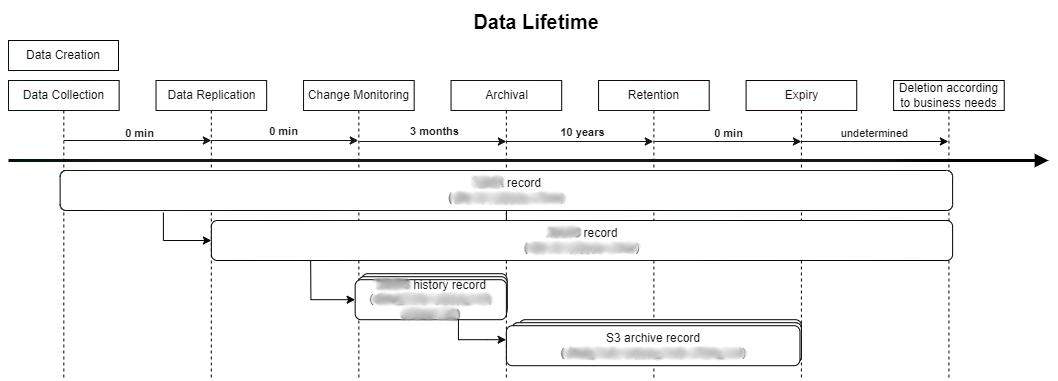
\includegraphics[width=\textwidth]{images/data_lifecycle_blurred.png}
            \caption{Duomenų gyvavimo ciklo diagrama}
            \label{fig:data_lifecycle}
        \end{figure}
        
    }
    \row

    \veikla{Gairių / dokumentacijos kūrimas}
    \aprasymas{
        % Issue URL: https://github.com/onlyidev/bachelor.practice/issues/9
        Specifinių aplikacijos duomenų archyvavimo panaudos atvejis su pasirinkta technologija dar nebuvo dokumentuotas vidinėje organizacijos dokumentų sistemoje, tad kūrimo fazės metu analizuota S3 dokumentacija, geriausios praktikos \cite{AmazonSimpleStorage} bei jomis remiantis priimti sprendimai (pvz.~duomenų kategorizavimo strategija) buvo suglaudinti ir aprašyti į S3 naudojimo gairių dokumentą. Taip pat sukurtas ir polapis sistemos (aplikacijos) dokumente, aprašantis konkretaus sprendimo įgyvendinimą.
    }
    \rezultatai{
        Paruoštos S3 naudojimo gairės, panaudos atvejis dokumentuotas. Dokumentai patalpinti organizacijos vidinėje sistemoje.
    }
    \row

    \veikla{Testavimo ir produkcijos aplinkų paruošimas}
    \aprasymas{
        \begin{itemize}
            \item Užpildytas \SD~dokumentas infrastruktūros komandai su reikalavimais paruošti
                  testavimo aplinkai tinkamą \textit{S3 on-prem} duomenų saugyklą. Testavimo aplinkai
                  numatyti vidutiniai saugyklos dydžio reikalavimai, duomenų gyvavimo ciklas sutrumpintas iki 6 mėn., programų sistemų kūrėjams suteikiama tik duomenų peržiūros teisė \angl{read-only, RO}.
            \item Užpildytas \SD~dokumentas infrastruktūros komandai su reikalavimais paruošti
                  produkcinei aplinkai tinkamą \textit{S3 on-prem} duomenų saugyklą. Produkcinei aplinkai
                  numatyti dideli (palyginus su esamu duomenų kiekiu) saugyklos dydžio reikalavimai, prieiga apribota tik techniniam vartotojui (aplikacijai).
            % Issue URL: https://github.com/onlyidev/bachelor.practice/issues/8
            \item Užpildytas \SD~dokumentas infrastruktūros komandai su reikalavimais sukurti aukšto lygio S3 kategorijas \angl{S3 buckets} \cite{AmazonSimpleStorage} paruoštose aplinkose.
            \item Aplikacijos konfigūracijose užpildyti S3 parametrai.
        \end{itemize}
    }
    \rezultatai {
        \begin{itemize}
            \item Paruoštos testavimo ir produkcinė saugyklos aplinkos.
            \item Gauti \textit{RO} prisijungimo duomenys į testavimo aplinką.
            \item Aplinkose paruoštos aukšto lygio S3 kategorijos.
        \end{itemize}
    }
    \row

    \veikla{Archyvavimo proceso įgyvendinimas}
    \aprasymas{
        \begin{itemize}
            \item Archyvavimo proceso komponento programavimas.
            \item Archyvavimo proceso modulių testų rašymas.
            \item Nuolatinio \angl{scheduled} naktinio proceso konfigūravimas.
            \item Užpildytas \SD~dokumentas monitoringo komandai su reikalavimais produkcinėje aplinkoje paruošti naktinio archyvavimo proceso stebėjimą pagal apibrėžtus nefunkcinius reikalavimus.
        \end{itemize}
    }
    \rezultatai{
        Įgyvendintas archyvavimo procesas, paruošti automatiniai monitoringo pranešimai, jei netenkinami nefunkciniai proceso reikalavimai. 
    }
    \row

    \veikla{Vartotojo sąsajos kūrimas}
    \aprasymas{
        % Issue URL: https://github.com/onlyidev/bachelor.practice/issues/7
        Archyvų peržiūros vartotojo sąsaja pasirinkta įgyvendinti kaip naują puslapį jau esamoje sąsajoje, sekančioje MVC \textit{(Model-View-Controller)} \cite{krasner1988description} šabloną.
    }
    \rezultatai{
        Sukurta vartotojo sąsaja, įgyvendintanti su susijusius funkcinius reikalavimus.
        % TODO(!Data): Add UI images 
        % Issue URL: https://github.com/onlyidev/bachelor.practice/issues/6
    }
    \row
    
    \veikla{Sprendimo pristatymas}
    \aprasymas{
        Įgyvendinto sprendimo, vartotojo sąsajos bei S3 naudojimo gairių pristatymas skyriaus kolegoms. 
    }
    \rezultatai{
        Skyriaus kolegos informuoti apie problematiką, priimtus bei įgyvendintus sprendimus.
    }
    \row

\end{activities}